\documentclass[12pt]{article}
\usepackage{amsmath,graphicx,amssymb,latexsym,epsfig,tabularx,setspace,verbatim,epstopdf,subfigure,xspace,setspace,todonotes}
\usepackage[margin=1in]{geometry}
\usepackage{sectsty}
\usepackage{natbib}
\usepackage{hyperref}

\def\eps{$\epsilon$\xspace}
\def\minpts{\emph{minpts}\xspace}
\def\dbscan{\textsc{Dbscan}\xspace}
\def\optics{\textsc{Optics}\xspace}
\def\vdbscan{\textsc{VariantDbscan}\xspace}


\begin{document}
\title{VariantDBSCAN: Maximizing Clustering Throughput}
\author{Mike Gowanlock\\ MIT Haystack Observatory\\ gowanloc@mit.edu}
\date{}
\maketitle

\tableofcontents

\section{Introduction}
\dbscan \cite{ester1996density} is a popular algorithm for clustering spatial data. The algorithm takes as input two parameters: \eps and \minpts, which define a neighborhood radius and density threshold to determine if points belong in a cluster.  The algorithm works by chaining points together, thus making it good for detecting clusters of arbitrary shape. Futhermore, it does not output a predefined number of clusters, making it an unsupervised approach.

Given that researchers typically need to execute \dbscan multiple times with different parameters, \vdbscan uses multiple optimizations to improve parallel clustering throughput.  In short, a variant is the definition of the two parameters that are taken as input into \dbscan. \vdbscan exploits data reuse between variants, reduces memory access overhead through efficient indexing of the points in the dataset, and schedules threads to variants to maximize data reuse between variants. See our paper \cite{Gowanlock2016} for more information about the optimizations. This code is a production version and does not contain all of the scheduling heuristics and cluster reuse approaches as described in \cite{Gowanlock2016}, as we selected the optimizations that performed the best in our experimental evaluation to limit the number of configuration options and parameters required to install and run \vdbscan.


\section{Installation}
We have included both C/C++ and Python interfaces to run \vdbscan.  Both of these use a common shared library developed in C++ that must be compiled on the system before use. For the python installation, there are two options, either install manually or use the pip package manager. A roadmap of instructions is given below depending on your preferred installation.

\begin{itemize}
\item C/C++: All instructions in Section~\ref{sec:sharedlib}, then Section~\ref{ref:cInterfaceInstall}.
\item Python (manual): All instructions in Section~\ref{sec:sharedlib}, then Section~\ref{sec:pymanual}.
\item Python (pip install): Make sure you meet the requirements in Section~\ref{sec:sharedlib_req}, then Section~\ref{sec:pypip}.
\end{itemize}

\subsection{Shared Library}\label{sec:sharedlib}
\subsubsection{Requirements}\label{sec:sharedlib_req}
The shared library, \texttt{libSharedVDBSCAN.so}, has been compiled and run using standard libraries, compilers and Linux operating system as outlined below.  We have included the versions of the software we used when compiling the shared library.  

For Mac OSX users, the code has been compiled using the python manual installation under OSX v.10.12. However, you must install g++ and OpenMP. At the time of writing, OSX v.10.12 and potentially other versions do not support LLVM/OpenMP.
\begin{enumerate}
\item Ubuntu (14.04.3)
\item GNU g++ (4.8.4)
\item OpenMP for multithreading (3.1, part of g++ installation)
\end{enumerate}

\subsubsection{Compile Options}\label{sec:sharedlib_compileopt}
There are two configuration options that can be modified in the \verb|makefile|:
\begin{enumerate}
\item \verb|SEARCHTHREADS| Default value: 4. \\This should be set to some number up to the number of cores on your machine.  This is the maximum number of threads that will concurrently cluster the variants.
\item \verb|libpath| Default value: \verb|/usr/local/lib/| \\This is the location of the shared libraries on your system. When compiling the shared library, the \verb|makefile| will copy the library to this location.
\end{enumerate}

\subsubsection{Installation}\label{sec:sharedlib_install}
To install the shared library, simply navigate to the src directory and type the following: \verb|sudo make libSharedVDBSCAN.so|

Note: you need to use \texttt{sudo} so the \verb|makefile| can copy the library into \verb|libpath|. However, if you do not have permissions, \verb|libSharedVDBSCAN.so| will be in the src directory, and you can link to it as you see fit. 


\subsection{C++ Interface}\label{ref:cInterfaceInstall}
In the \texttt{src} directory, the code in \verb|c_test_prog.cpp| is an example test program that uses the shared library. To compile this program, type: \verb|make c_test_prog|. This assumes that \verb|libSharedVDBSCAN.so| has been successfully copied into \verb|libpath|.  Otherwise, modify \verb|makefile| to link to the location of \verb|libSharedVDBSCAN.so|.



\subsection{Python Interface: Manual Installation}\label{sec:pymanual}
In the \texttt{src} directory open \texttt{variantdbscan.py} and modify \verb|lib_path| to be the directory that contains \texttt{libSharedVDBSCAN.so}.  The python wrapper, \texttt{variantdbscan.py}, links to the shared library.
The following code in \texttt{variantdbscan.py} should be modified according to the comments:

\noindent \verb|# Get library path|\\
\noindent \verb|# Use the following line if installed by pip|\\
\noindent \verb|lib_path = os.path.dirname(os.path.realpath(__file__)) + '../'|\\
\noindent \verb|# Otherwise, comment out the above line and|\\
\noindent \verb|# uncomment the following line, adjusting path as necessary|\\
\noindent \verb|# lib_path = '/usr/local/lib/'|

\subsection{Python Interface: Using the Pip Package Manager}\label{sec:pypip}
To install via pip, the environment variable \verb|NTHREADS| variable should be set to some number up to the number of cores on your machine.  This is the maximum number of threads that will concurrently cluster the variants. If you do not set \verb|NTHREADS|, it will default to 4. \\

\noindent To install, type: \verb|sudo NTHREADS=4 pip install vdbscan|


\section{Usage}\label{sec:sharedliboverview}
The shared library is called \verb|libVDBSCAN()|. The function signature is as follows:\\
\texttt{int libVDBSCAN(double * inputx, double * inputy, unsigned int datasetSize, \\double * inputEpsilon, unsigned int * inputMinpts, unsigned int numVariants,\\ int MBBsize, unsigned int * retArr, bool verbose);}\\
\\Explanation of the variables:

\begin{itemize}
\item \texttt{double * inputx} and \texttt{double * inputy} - Dataset values in two dimensions as two arrays.
\item \texttt{unsigned int datasetSize} - Number of points in the dataset (size of the length of \texttt{inputx} and \texttt{inputy}).
\item \texttt{double * inputEpsilon} and \texttt{unsigned int * inputMinpts} - Arrays of variant \eps and \minpts values.
\item \texttt{unsigned int numVariants} - The number of variants to be clustered (size of the length of \texttt{inputEpsilon} and \texttt{inputMinpts}).
\item \texttt{int MBBsize} - The number of points per minimum bounding box for the R-tree index (Default value: 70).
\item \texttt{unsigned int * retArr} - An array containing the result set.  Each point in the dataset is assigned a cluster id. This array is the cluster ids of points for each variant. The length of this array is:  \texttt{datasetSize} $\times$ \texttt{numVariants} (or $|D|\times|V|$ in \cite{Gowanlock2016}).
\item \texttt{bool verbose} - Flag to turn on or off optional output.
\end{itemize}


\texttt{retArr} contains the results across all variants. The cluster id is given for each point, where an id of 0 indicates that it is a noise point (not in a cluster).


\subsection{C++}
First, you must compile \verb|c_test_prog.cpp| outlined in Section~\ref{ref:cInterfaceInstall}. Here, we go through the example clustering in the test program. 

The following variables are set to cluster two variants ($\epsilon=1.0$, $minpts=10$) and ($\epsilon=0.5$, $minpts=12$).

\begin{itemize}
\item \verb|dataset| -- set to \verb|test_dataset.csv|
\item \verb|numVariants| -- set to 2
\item \verb|inputEps| -- set to [1.0, 0.5]
\item \verb|inputMinpts| -- set to [10, 12]
\end{itemize}


Run the program: \verb|./c_test_prog| 


The program will output the results, as shown in Appendix~\ref{ex_output}. A plot of the results of both variants is also shown.



\subsection{Python}
The python test program in the \texttt{src} directory is called \verb|variant_example.py|. First, depending on how the \vdbscan interface was installed (manually or through pip), the correct import statement should be selected:

\noindent When using the pip installed version:\\
\texttt{from vdbscan import VariantDBSCAN\\}

\noindent When using the manually installed version:\\
\texttt{from variantdbscan import VariantDBSCAN\\}


The following variables are set to cluster two variants ($\epsilon=1.0$, $minpts=10$) and ($\epsilon=0.5$, $minpts=12$).

\begin{itemize}
\item \verb|data = pd.read_csv("test_dataset.csv", header=None,names=['x','y'])|
\item \verb|eps = np.array([1, 0.5])|
\item \verb|mp = np.array([10, 12])|
\end{itemize}


Run the program: python \verb|variant_example.py|

The program will output the results, as shown in Appendix~\ref{ex_output}. A plot of the results of both variants is also shown.

\section{Source Code Overview}
While this document is intended primarily for those wanting to use the source code for clustering, we outline the structure of the code.  The reader intending to make algorithmic changes to the code should first be very familiar with the \dbscan algorithm and then the \vdbscan paper~\cite{Gowanlock2016}.  See the doxygen directory for the html and pdf versions of the code. The callgraph for \texttt{libVDBSCAN} is probably the most useful.

The flow of the program \texttt{libVDBSCAN} (in \texttt{main.cpp}) is outlined as follows.  First, the variants are imported and marshalled into a vector. This vector is sorted based on the Greedy scheduling heuristic.  Next, the dataset is imported from the arrays into a vector. The data is then binned spatially such that data points nearby each other are close to each other in memory, thus improving locality, and allowing for the R-tree to index points together in compact MBBs.  The R-tree index is initialized, where the leaf nodes are defined by MBBs that contain multiple points.  To allow for the individual data points to be accessed from the R-tree, a lookup array is used. The MBBs that  represent multiple points are inserted into the R-tree. Next, another R-tree index is initialized that indexes each point in its own MBB. This index is not used for \eps-neighborhood searches, rather it is used in the process of expanding a cluster to reuse data from a previously executed variant.  The DBScan objects are initialized, where each object corresponds to a single variant. The scheduler is initialized which creates a job queue to assign variants to threads in the Greedy scheduling order. Furthermore, the scheduler determines whether a completed variant can be used as input to cluster a variant yet to be processed.  

The implementation uses OpenMP. A thread executes a single loop iteration, where the thread is assigned a variant to process by the scheduler. Also, the scheduler determines if a given variant assigned to a thread can reuse any completed variants. Two execution pathways can occur: 1) If there are no variants that can be reused for a given variant, then the variant is clustered from scratch; or 2) if the variant can reuse the results from a completed variant, then it will use the previous cluster assignments as input into the algorithm. Thus, a single thread executes a single variant (whether clustering from scratch or reusing data from a previous variant). After all of the variants have been clustered, the result set array is returned.  To return the data, two transformations have to occur. First, the dataset needs to be mapped to its original ordering (recall that we reorder the data to improve locality and for indexing purposes). Secondly, the variant results (assignment of points to clusters) need to be reordered to be the same order that was sent to the function. 



The source code contains many comments to help the reader understand the program. The code has three major classes that will be described in the following subsections. 
\begin{itemize}
\item RTree -- A spatial index to efficiently find the data points in the dataset, primarily for $\epsilon$-neighborhood searches.
\item schedule -- Determines the ordering in which the variants are executed.
\item DBScan -- Each DBScan object executes a single variant.
\end{itemize}

\subsection{R-Tree}
The R-Tree is a spatial index used to find the data points in the dataset (\eps-neighborhood searches) and is used in the process of reusing data from the output of one variant as input into another. 

A single R-tree is constructed that contains a number of minimum bounding boxes (MBB) that contain points spatially nearby each other in the dataset. The number of points per MBB is set by \texttt{MBBsize}, described in Section~\ref{sec:sharedliboverview}.   Putting multiple points in a single MBB reduces tree depth at the expense of more filtering overhead.  When clustering, this R-tree is traversed by multiple threads to perform the \eps-neighborhood searches in the algorithm for different variants.

Another R-tree is constructed that indexes each point in its own MBB. This is used when taking the clusters from the output of one variant, and using it as input to ``short circuit'' the clustering of another variant. That is, the data points belonging to one cluster may be common to two variants and thus expensive \eps-neighborhood searches can be avoided. See \cite{Gowanlock2016} for more information.

Pointers to two R-tree indexes are taken as input to DBScan objects.

\subsection{Scheduling}
To allow for data reuse between variants, the output of one variant contains cluster assignments that may apply to another variant. In short, clusters with smaller values of \eps can be used as seeds to create clusters that have higher values of \eps. In order to maximize the chances of data reuse between variants, the scheduling algorithm creates an ordering of the execution of variants as a function of the \eps and \minpts values.  This is conflated with the number of threads used. If variants are still waiting to execute in the work queue and a thread is idle, the thread will be assigned a variant to process where the two execution pathways can occur (cluster from scratch or reuse data).  The Greedy schedule in~\cite{Gowanlock2016} is used. 

\subsection{DBScan}

Initializing the object takes as input: the dataset, the variant parameter values: \eps and \minpts, an R-tree for \eps-neighborhood searches, an accompanying lookup array into the dataset, and a high resolution R-tree which is utilized when expanding a cluster when reusing data between variants. As mentioned above, two execution pathways can occur: 1) If there are no variants that can be reused for a given variant, then the variant is clustered from scratch; or 2) if the variant can reuse the results from a completed variant, then it will use the previous cluster assignments as input into the algorithm.

If the variant is clustered from scratch, then the class executes the function\\ \texttt{algDBScanParallel()}. This is the standard \dbscan algorithm with the index optimization that uses an R-tree with multiple points per MBB. Note that a single thread executes a single variant, and multiple threads concurrently cluster different variants.

If the variant can reuse data from a previously completed variant, then\\ \texttt{assignPointsToPredefinedCluster()} is executed.  This method takes as input the id of the previously finished variant object. Through a pointer to the object, the variant to be processed has access to the cluster assignments of all of the points in the completed variant. With this information, clusters can be reused as the points belonging to one cluster are guaranteed to be common in another cluster (based on the criteria outlined in~\cite{Gowanlock2016}). \texttt{assignPointsToPredefinedCluster()} has a few major steps, as follows:

\begin{enumerate}
\item A list of clusters is obtained from the previously completed variant.
\item These clusters are prioritized using the density cluster reuse heuristic.
\item The list of candidate clusters to expand are expanded by adding new points to the cluster with \eps-neighborhood searches.  This continues until all of the points in the candidate clusters have been visited or the candidate clusters have been destroyed through the process of reuse.
\item Finally, any points in the dataset that have not been visited, are clustered (they may have been noise points in the previously completed variant, but may form a cluster in the new variant). 
\end{enumerate}


\section*{ACKNOWLEDGMENTS}
We acknowledge support from NSF ACI-1442997.



\appendix
\section{Example Output}\label{ex_output}

Data is in the format: point id, x value, y value, cluster assignment. Cluster id 0 is a noise point. The dataset, \verb|test_dataset.csv| has 225 points. Plots of the assignment of points to clusters is shown in Figures~\ref{fig:Variant0}~and~\ref{fig:Variant1}, where colors indicate different clusters.

\noindent\textbf{Output:} 

\noindent Variant: 0, Epsilon: 1.000000, minpts: 10
\\0, 6.689900, -0.131300, 2
\\1, -3.989800, -1.113700, 1
\\2, 4.268700, -0.687100, 2
\\3, -6.031600, 1.570700, 1
\\4, 4.704300, -0.315900, 2
\\5, -3.534000, -1.283700, 1
\\6, -6.767100, 1.524200, 1
\\7, 3.293400, -2.245800, 2
\\8, -5.150900, -0.269400, 1
\\9, -4.670700, -0.986800, 1
\\10, 5.630800, 0.360500, 2
\\$\ldots$
\\215, 3.758700, 5.909100, 0
\\216, -5.874500, 3.702000, 0
\\217, -3.680800, -0.943700, 1
\\218, -4.298700, -0.441000, 1
\\219, 3.337700, -2.005900, 2
\\220, -6.111300, 1.477300, 1
\\221, 5.133000, 0.894600, 2
\\222, 6.219200, 0.936800, 2
\\223, -4.717400, -0.258900, 1
\\224, 6.067300, 0.611400, 2\\

\noindent Variant: 1, Epsilon: 0.500000, minpts: 12
\\0, 6.689900, -0.131300, 0
\\1, -3.989800, -1.113700, 1
\\2, 4.268700, -0.687100, 2
\\3, -6.031600, 1.570700, 1
\\4, 4.704300, -0.315900, 2
\\5, -3.534000, -1.283700, 1
\\6, -6.767100, 1.524200, 0
\\7, 3.293400, -2.245800, 0
\\8, -5.150900, -0.269400, 1
\\9, -4.670700, -0.986800, 1
\\10, 5.630800, 0.360500, 2
\\$\ldots$
\\215, 3.758700, 5.909100, 0
\\216, -5.874500, 3.702000, 0
\\217, -3.680800, -0.943700, 1
\\218, -4.298700, -0.441000, 1
\\219, 3.337700, -2.005900, 0
\\220, -6.111300, 1.477300, 1
\\221, 5.133000, 0.894600, 2
\\222, 6.219200, 0.936800, 2
\\223, -4.717400, -0.258900, 1
\\224, 6.067300, 0.611400, 2


\begin{figure}[htp]
\centering
            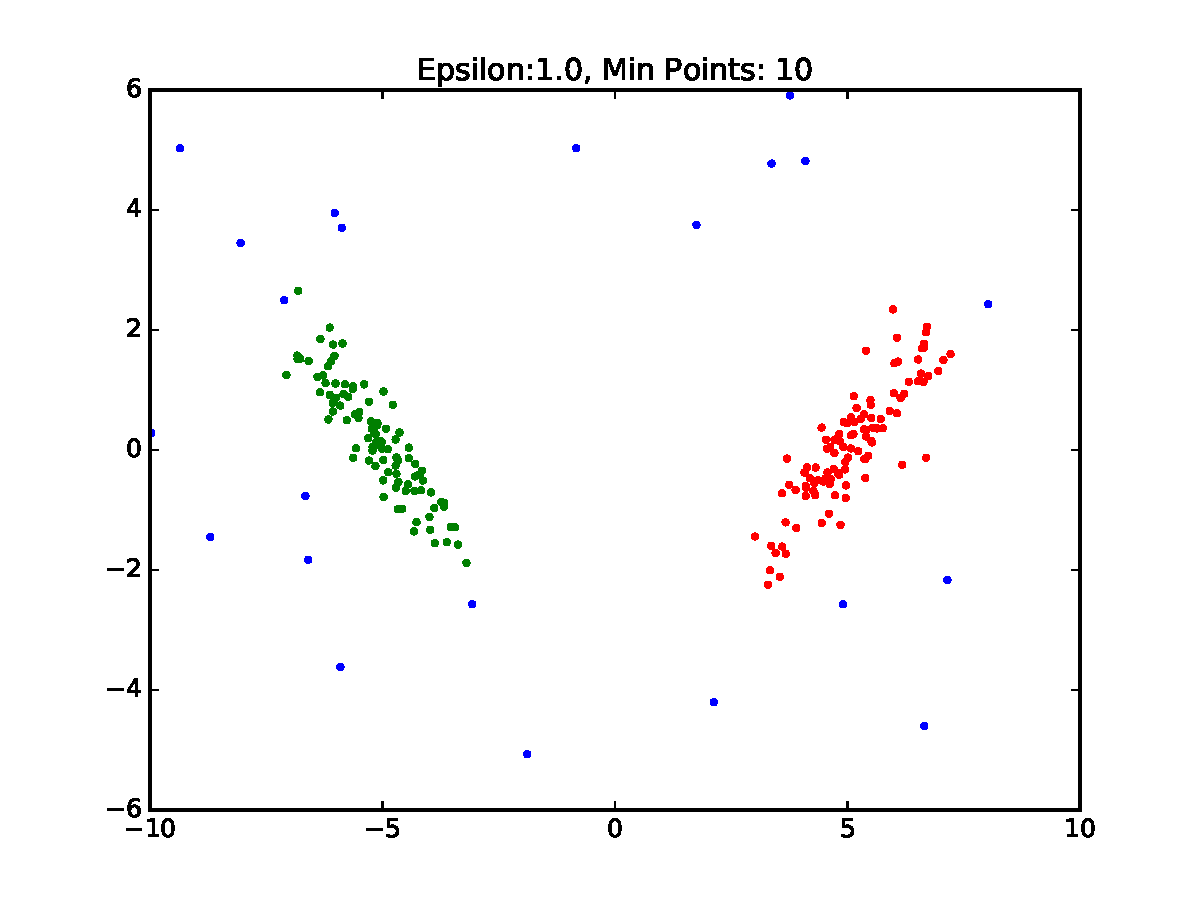
\includegraphics[width=0.7\textwidth]{images/test_results_0.pdf}   
    \caption{Plot of the clusters in the dataset with $\epsilon=1.0$ and $minpts=10$. Two clusters are detected (green, red) and noise points are blue.}
   \label{fig:Variant0}
\end{figure}

\begin{figure}[htp]
\centering
            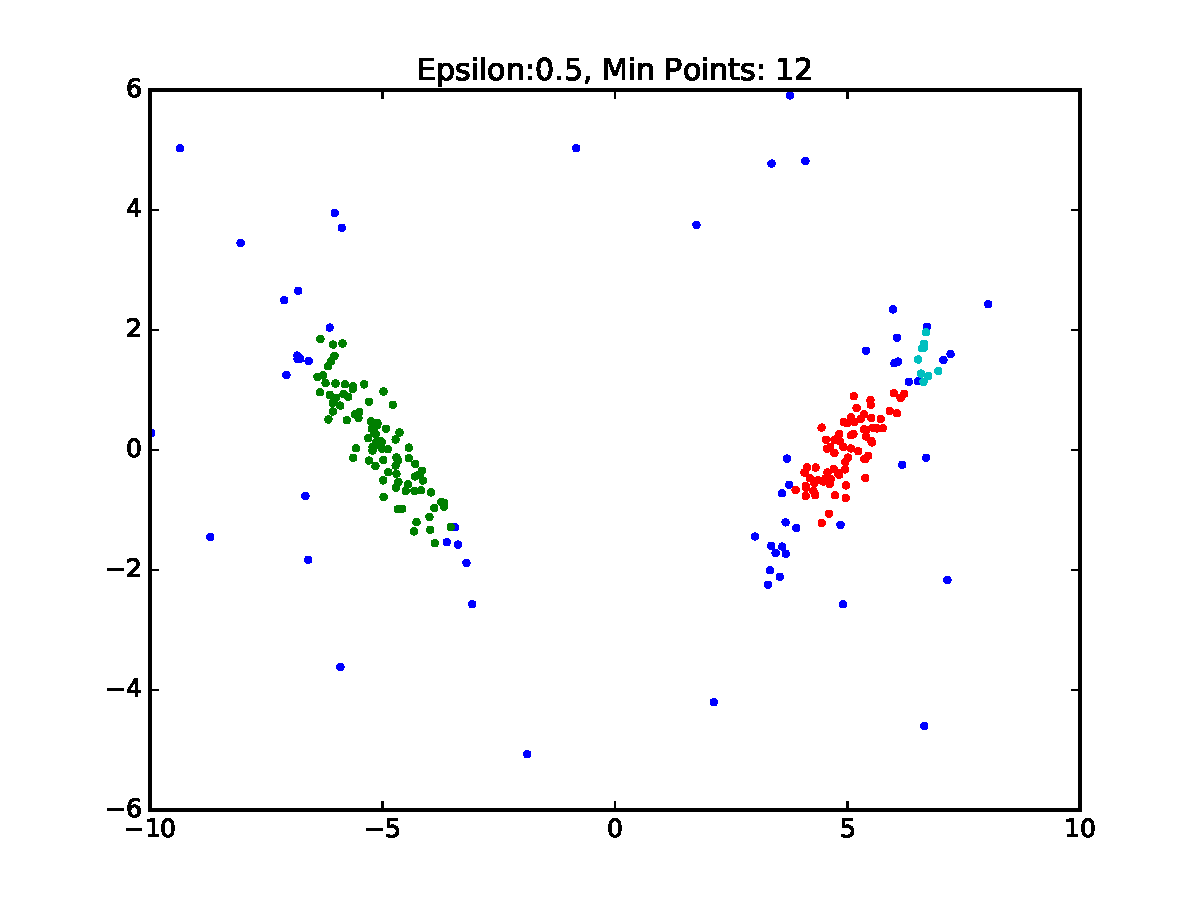
\includegraphics[width=0.7\textwidth]{images/test_results_1.pdf}   
    \caption{Plot of the clusters in the dataset with $\epsilon=0.5$ and $minpts=12$. Three clusters are detected (green, red, cyan) and noise points are blue.}
   \label{fig:Variant1}
\end{figure}

\bibliographystyle{plain}
\bibliography{bibliography}

\end{document}

